\section{Prinsipiell løsning}
\label{prinsipiellLoesning}

%Her kan du skrive om prinsipiell løsning

For å designe en terning må man ha et tilfeldig tall man kan dekode til øyne på en terning. Som sett i \ref{fig:Fig1} så vil terningen i dette designnotatet bestå av en teller som teller fra 1 til 6 i klokkefrekvensen til FPGAen, den vil kun stoppe ved et signal som kommer fra en knapp brukeren kan trykke på. Dette vil ikke gi et helt tilfeldig tall, men hastigheten på systemet er så høy at man kan annta at systemet vil stoppe på en tilfeldig verdi. Som vist i \ref{fig:Fig1} Så er det lagt inn register etter telleren for å lagre terningkastets verdi. For så ha en dekoder som dekoder signalet til LED matrisen. 

\begin{figure}[htbp]
  \centering
  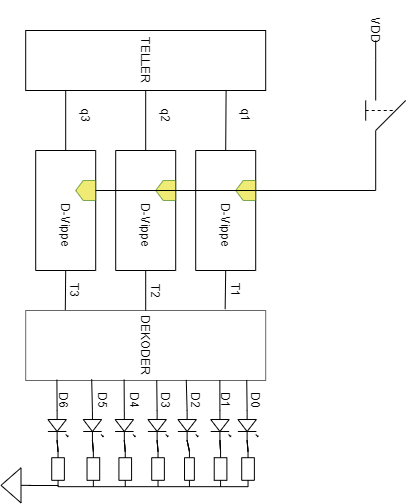
\includegraphics[width=0.6\textwidth,angle = 90]{Bilder/overordnet.png} 
  \caption{Prinsipiell overordnet løsning}
  \label{fig:Fig1}
\end{figure}
